\documentclass[twocolumn]{revtex4}

\usepackage[]{graphicx}

\begin{document}

\title{
Journal Article
}

\author{Nicole McAdams}
\affiliation{Siena College, Loudonville, NY}

\date{\today}

\begin{abstract}
Could a human escape a velociraptor if he/she got a head start? This is the question to answer using different algorithms.  First, you need to find the position in which the velociraptor catches up with the human, if the human has a 30 meter head start.  At two seconds, both creatures have traveled 36 meters.  Knowing that the velociraptor will begin to attack within one meter of the human, you need to find what time/position it will begin to lunge.  I found this time to be 1.93 seconds; the human has ran 35.79 meters and the velociraptor has ran 34.74 meters.  Once the velociraptor is in biting range, it has three chances to succeed.  The first attempt, there is a 20 percent chance it will bite you, then it falls to a 15 percent chance, and the final attempt has a 7 percent chance of a successful attack.  If the velociraptor doesn't bite you after the three tries, you have gotten away safely.  The chance of you getting away is about 63.5 percent.   

\end{abstract}

\maketitle 
$$ 'Raptor Attack$$

\section{Introduction} 

In order to plot the position vs. time graph, I have to figure out the position functions for both the human and velociraptor.  The formula I used to figure these out was $ x_f = x_o + v_ot $ This formula gives the final distance of the creature, depending on their initial position ($x_o$) and initial velocity multiplied by the amount of time it has been moving at this speed ($v_ot$).  The position function for the velociraptor is $ x_f =  18t $ and the position function for the human is $ x_f = 30 + 3t $.  When I plotted these functions, I got this graph: 

\begin{figure}[h!]
	\centering
	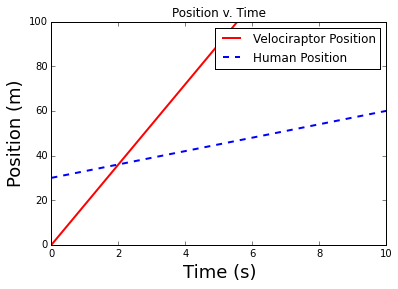
\includegraphics[width = .5\textwidth]{p v t graph 1.png}
	\caption{This is the Position vs. Time graph.  At the point the lines intersect, this is where the velociraptor and human are at the same position.  \label{ptoe}}
\end{figure}

\subsection{Explaining code}
To decide the x-coordinates, I had to generate 1001 points between zero seconds and 10 seconds.  These points are evenly spaced.  For the y values, I set y equal to the position functions, which plug in x values to create coordinates.  

\section{When does the 'raptor catch up ?}
Although you can estimate when the human and 'raptor intersect based on the graph, a more exact answer can be derived through code.  My algorithm loops through both sets of values for the human positions and velociraptor positions.  When the similar position is located, the computer prints out the x (time) value that coincides with the position, along with the position value.  

\subsection{Solving Algebraically}
$$ x_f = x_o + v_ot , x_f = v_ot $$ 
$$ 30 + 3t = 18t $$ 
$$ t = 2 $$

\section{When can the 'raptor attack?}
We are told that a velociraptor will begin to strike when it is one meter away from the human;  the task is to find out what time this will happen.  To do this, I had to loop over both sets of data and figure out the time that the difference between the positions was one meter.  To get one answer, I had to specify that the distance had to be greater than one meter and less than 1.1 meters.  When this spot is located, the computer prints the time of this occurrence, along with the positions of both the human and the velociraptor. The time was 1.93 seconds, the distance the human traveled was 35.79 meters, and the distance the velociraptor traveled was 34.74 meters.  The graph of this plot is: 

\begin{figure}[h!]
	\centering
	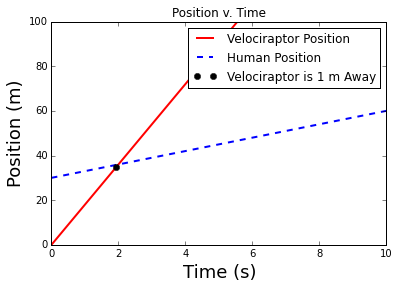
\includegraphics[width = .5\textwidth]{p v t graph 2.png}
	\caption{This is the Position vs. Time graph.  The black dot located the point at which the velociraptor is one meter away from the human.  \label{ptoe2}}
\end{figure}

\subsection{Explaining code}
To get the x and y coordinate, I used the same setup as the previous graph.  The reason i chose to create 1001 x-points is because the more points in the x-axis, the closer the exact value for the time the 'raptor is one meter away.  In order to plot the black dot on the graph, I had to figure out the point at which this occurred, by doing the previous explained process.  Then I plotted that exact point, (1.93,34.74).

\subsection{Solving Algebraically}
$$ x_H - x_V = 1 $$ 
$$ 30 + 3t - 18t = 1 $$ 
$$ t = 1.93 $$ 

\section{Will you get away?}
When the 'raptor begins to strike, there is a 20 percent chance the raptor will bite you.  If the raptor misses, it gets frustrated and there is only a 15 percent chance the 'raptor will bite you.  If you get away, the 'raptor strikes one more time with a 7 percent chance of succeeding.  If you get away the third time then you are safe.  To figure out the chance of survival, I had to create a "for" loop which would pass through 100000 points, created randomly.  The point passes through the three bite scenarios.  The amount of points that survive are divided by the number of points tested and multiplied by 100.  This outcome gives the probability of survival: roughly 63.5 percent.  

\subsection{Explaining code}
The first step was to generate 100000 random points between zero and one.  Then, in the "for" loop, I called one random number to pass through the system.  The first step is to see if the number is larger than .2; if it is then it survived the first bite.  If it survived the first bite, it passes through the second "if" statement to see if it is larger than .15.  If it's larger than it survives the second bite.  The number is then passed to the last "if" statement to see if its larger than .07 and if it is then it survived the 'raptor attack.  This process continues for 99999 more points.  The points that passed through this entire loop are totaled.  The total number is placed over the number of original points and multiplied by 100.  



\end{document}
